\begin{frame}
\frametitle{Гипотезы о коррупции}
\begin{itemize}
	\item Механизм 1: Спонсирование предвыборной компании одного из кандидатов
	\item Механизм 2: Взятки для выигрыша тендеров после выборов 
\end{itemize}
Тестирование гипотез: проверяется теснота связи между выводом средств во время выборов и коррумпированностью региона. 
\begin{center}
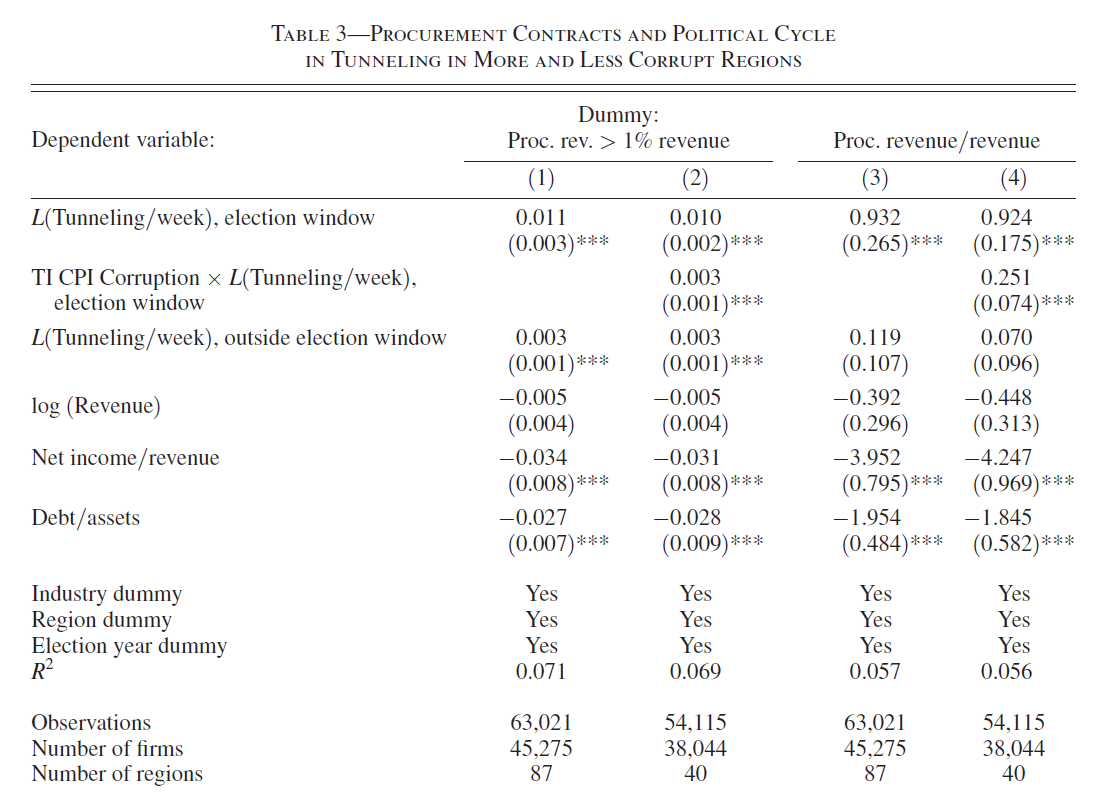
\includegraphics[scale=0.17]{images/kek4}
\end{center}
\end{frame}

\begin{frame}
\frametitle{Гипотезы о коррупции}
\begin{itemize}
	\item Получен устойчивый результат, что вывод средств во время выборов и получение госконтрактов связаны с уровнем коррупции в регионе
	\item Таким образом, подтвердилась гипотеза, что коррупция является механизмом влияния выборов на объем выводимых денег  
\end{itemize}
\end{frame}

\begin{frame}
\frametitle{Гипотеза влияния предвыборной активности на цикл вывода денег}
\begin{itemize}
	\item В регрессию включены объемы входящий транзакций за несколько предыдущих периодов, что уже должно значительно снизить влияния этого фактора на $\gamma$
	\item Оценивается регрессия того же вида, но в левой чисти стоят трансферы в пользу законных фирм, не связанных с предвыборной деятельностью
\end{itemize}
\end{frame}

\begin{frame}
$\beta^1_m + \beta^2_m$:
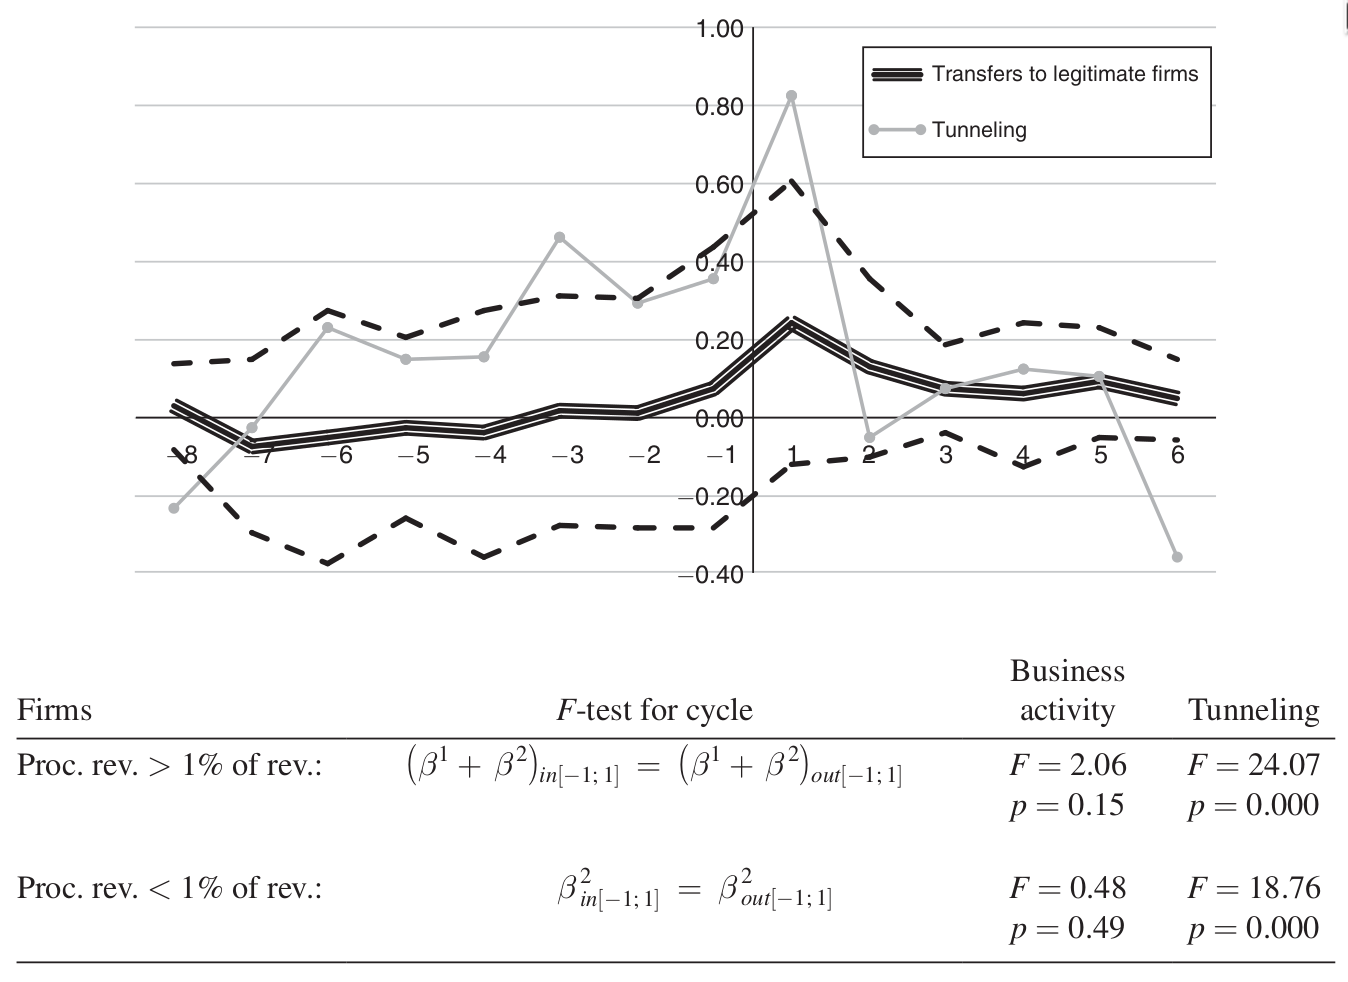
\includegraphics[scale=0.25]{images/legit_trans}
\end{frame}

\begin{frame}
\frametitle{Чувствительность вывода к доходам от госзаказов}
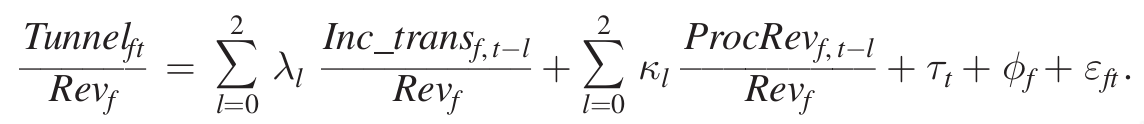
\includegraphics[scale=0.3]{images/tunnelling_from_procurement}
$k$ большие, но это ожидаемо - должностные лица могут требовать взятки после выигрыша тендера
\end{frame}

\begin{frame}
Но в самих доходах от госзакупок политического цикла нет:
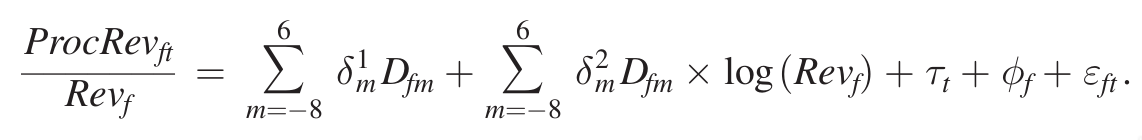
\includegraphics[scale=0.3]{images/tunnelling_from_procurement2}\\
\vspace{3mm}

$\delta^1_m$:\\
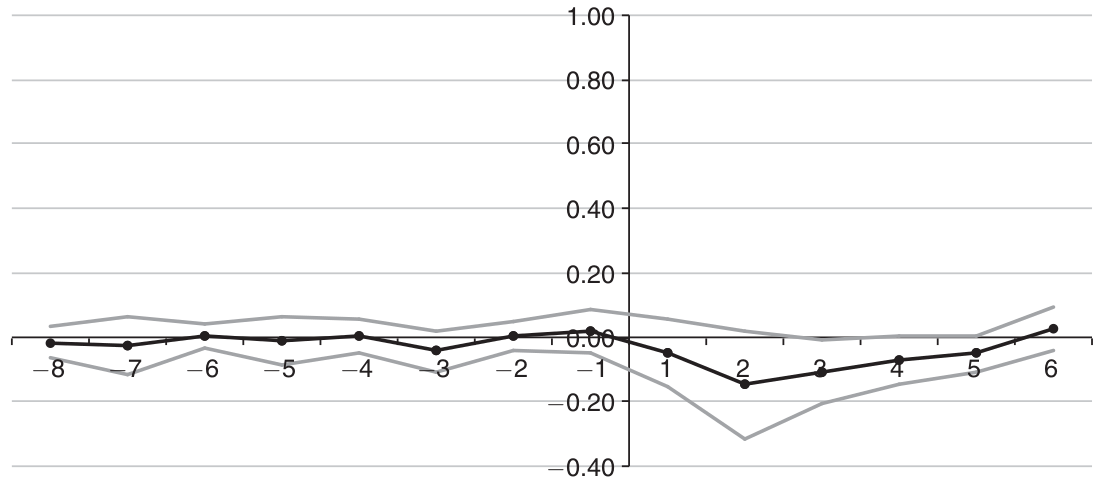
\includegraphics[scale=0.25]{images/tunnelling_from_procurement3}
\vspace{3mm}

Также добавляют лаггированные $\frac{ProcRev_{ft}}{Rev_f}$ в основное уравнение - результаты оценки не меняются
\end{frame}

\begin{frame}
\frametitle{Политический риск}
Одна из возможных причин существования политического цикла - риск смены политики, наибольшим образом влияющий на фирмы, выполняющие гос. заказы.\\
\vspace{3mm}

Оцевидно, политический цикл в таком случае должен сильнее проявляться, когда исход выборов неизвестен\\
\vspace{3mm}
\end{frame}

\begin{frame}
\frametitle{Политический риск}
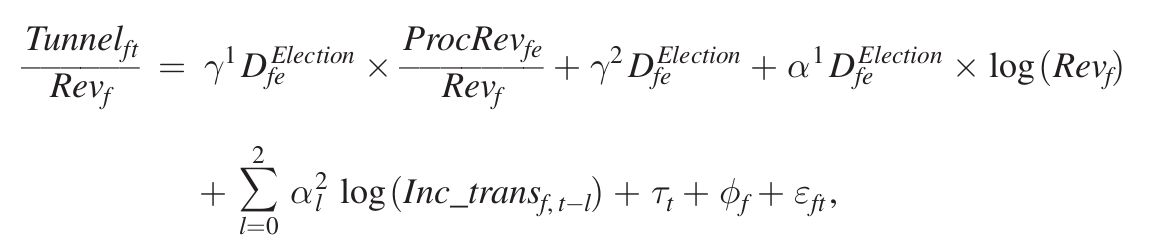
\includegraphics[scale=0.25]{images/prisk1}
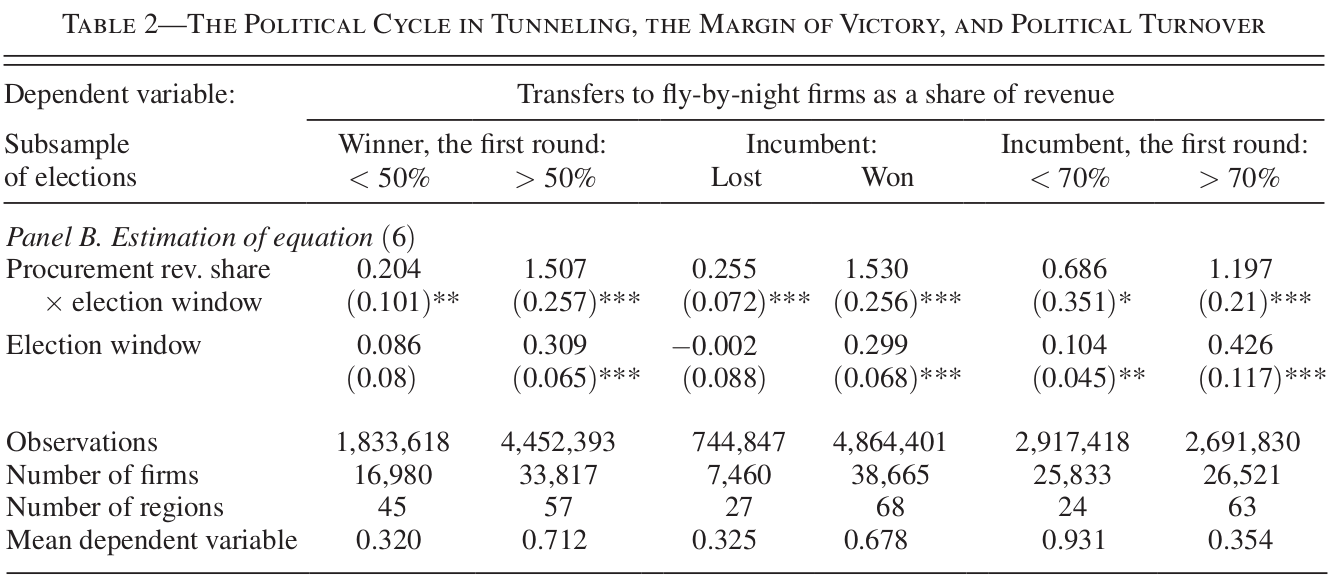
\includegraphics[scale=0.25]{images/prisk2}
\end{frame}